% used to distinguish the main document from the subdocument.
% if COMPLETE is defined subdocument will not declare begin and
%  end of document, and will not import packages.
% if COMPLETE is not defined, a subdocument can be compiled individually.
\def\COMPLETE{}

\documentclass[11pt]{article}

\usepackage{enumitem}
\usepackage{listings}
\usepackage{color}
\usepackage{graphicx}
\usepackage{epigraph}
\usepackage{courier}

\newenvironment{myAbstract}
  {%\clearpage           % we want a new page
   %\thispagestyle{empty}% no header and footer
   \vspace*{\stretch{1}}% some space at the top 
   \itshape             % the text is in italics
   \center
   %\raggedleft          % flush to the right margin
  }
  {\par % end the paragraph
   \vspace{\stretch{3}} % space at bottom is three times that at the top
   \clearpage           % finish off the page
  }
  
\def\changemargin#1#2{\list{}{\rightmargin#2\leftmargin#1}\item[]}
\let\endchangemargin=\endlist 

%Gummi|065|=)
\title{\textbf{Work Pay Calculator}}
\date{2018/10/04}
\author{Luca Parolari\footnote{luca.parolari23@gmail.com}}


\begin{document}

\maketitle
%\clearpage

\begin{myAbstract}
\textbf{Abstract}
\begin{changemargin}{2cm}{2cm}
\input{abstract.txt}
\end{changemargin}
\end{myAbstract}

\tableofcontents
\clearpage

\ifdefined\COMPLETE
\else
\documentclass[11pt]{article}

\usepackage{enumitem}
\usepackage{listings}
\usepackage{color}
\usepackage{graphicx}
\usepackage{epigraph}
\usepackage{courier}
\usepackage{hyperref}


\begin{document}
\fi


%%%%%%%%%%%%%%%%%%
% WPC
\section{WPC}

\subsection{What is}
\textit{Work Pay Calculator} has the objective to simplify the \textbf{management} of the work done in terms of hour, cost and profits. In other hands WPC is an application that smartly stores hours done for a work and allows to automatize the process of hours pay calculation and \textit{occasional performance}\footnote{This is an italian fiscal document that certifies work for someone.} emission.

\subsection{What is not}
WPC is not a management tool for fiscal things, futhermore, for now, it's not an hour marker in terms of real-time start and stop counter (see \ref{subsec:enhancements}).

\subsection{Features}
\begin{enumerate}[label=(\alph*)]
\item Light-weight, simple and easy to use.
\item Easily syncronizable with cloud services: only the executable and the data storage is needed. Data storage needs to be syncronized only if the SQLite engine is chosed.
\item CLI inteface, in order to focus the objective to the application functionalities.
\item Highly configurable: personalize environment variables and achieve your needs.
\item Default answer configuration. Lot of configurable default answers, avoing boring data typing.
\end{enumerate}

\subsection{Examples}
\textbf{Scenario 1}: today I've worked for a customer 6 hours: 3 of coding, 1 learing a new technology and 2 to publish the work online. What the hell, I have to register this things before I forget them.

No problem, open WPC and insert a new work in a way like this:

\begin{lstlisting}
wpc> work: today 14:30 17:30 true
wpc> work: km? [0]: 
wpc> work: add? [0]: 
wpc> work: registry? [General work]: I've coded the
pinco pallo project
wpc> Work inserted successfully!
\end{lstlisting}

And you can repeate this procedure any time you want to increase the datail of hours done in this day.

\ifdefined\COMPLETE
\else
\end{document}
\fi

%%%%%%%%%%%%%%%%%%
% Analisys
\section{Analisys}
This chapter will report the result of the project analisys, and its requirements.

\subsection{Requirements}
The system will be developed as a library written in Python (for educational purposes) with a minimal CLI\footnote{Command Line Interface}. The system will need a dababase, in this context SQLite will be chosen (for educational purposes again), however a strategy to make db engine interchangable could be adopted in later versions (see \ref{subsec:enhancements}).

The system should allow the user to:
\begin{enumerate}[label=(\alph*)]
\item Setup system variables, even if default values are setted. (see \textit{\ref{subsec:configuration}});
\item Manage clients;
\item Enter a new line of work with following data: 
\begin{enumerate}[label=\arabic*)]
\item Date of work;
\item Start and end time of work, or directly number of hours done;
\item Boolean production value: true if the work can be marked as production, false otherwise;
\item The kilometers done to reach the work place (if any);
\item An add value, if any extra outgoings;
\item Some notes, to mark down any noticeable data or to specify what the add value stands for;
\item A description of work done;
\end{enumerate}
\item Mark some dates as paid;
\item Allow registering forfait payments, that should be removed from the next bill;
\item Show some statistics:
\begin{enumerate}[label=\arabic*)]
\item Total hours done;
\item Total non-production hours done;
\item Total production hours done;
\item Total kilometers done;
\item Total add;
\end{enumerate}
This should be allowed for each paid "session", including not paid data as default.
\item Financial report:
\begin{enumerate}[label=\arabic*)]
\item Total hours profit;
\item Total non-taxable hours profit;
\item Total taxable hours profit;
\item Total kilometers cost;
\item Total add cost;
\item Total profit;
\item Total profit with fiscal elaboration (IVA, gross and net to pay). 
\end{enumerate}
Also this should be available for each paid "session", including not paid data as default.
\end{enumerate}

\subsection{Configuration}
\label{subsec:configuration}
The system needs some static parameters that can change in the future. The a configuration manager is needed to handle this requirement.

Configuration to handle are:
\begin{enumerate}[label=(\alph*)]
\item euro/hour value, i.e. how much an hour of work cost for the customer. For now, every hour has the same cost, but in future could be implemented a way to make some hours with a price and some other with other price;
\item kilometers/litre, in order to calculate how miny litres of gas are needed base on km done;
\item litre/euro, in order to calculate a possible value to expose as a cost (will be approximate);
\item IVA, the italian fistal number for taxes.
\end{enumerate}


\subsection{Enhancements}
\label{subsec:enhancements}
Here will be listed all programmate or desiderable changes to the project.

Programmed enhancements: \textit{none} for now.
To consider: 
\begin{enumerate}[label=(\alph*)]
\item Multiple database engine support;
\item Different hour cost based on work;
\end{enumerate}

\ifdefined\COMPLETE
\else
\documentclass[11pt]{article}

\usepackage{enumitem}
\usepackage{listings}
\usepackage{color}
\usepackage{graphicx}
\usepackage{epigraph}
\usepackage{courier}
\usepackage{hyperref}


\begin{document}
\fi


%%%%%%%%%%%%%%%%%%
% Design
\graphicspath{ {./images/} }

\section{Design}
This section will describe how the software is designed.

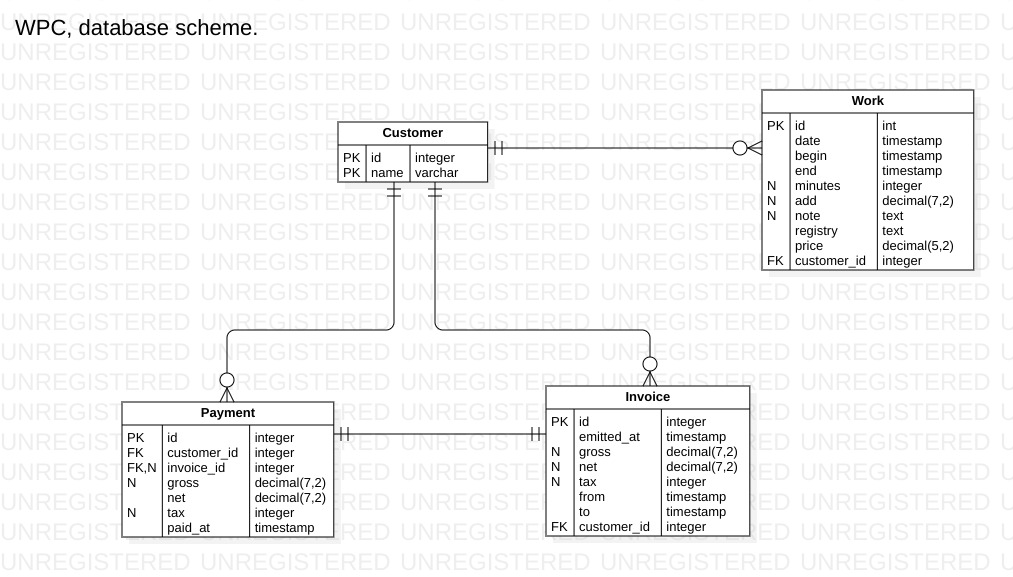
\includegraphics[scale=0.4]{wpc_data_model}

\subsection{CLI}
The command line interface is a foundamental tool: it allows the usage of the program without any complicance in UI design, however, even the CLI needs to be designed.

Commands for clients management:
\begin{lstlisting}
> cli show
> cli add <id>|<name>
> cli remove <id>|<name>
> cli switch <id>
\end{lstlisting}

Commands for work management:
\begin{lstlisting}
> (cli) work --filters column1=value1, column2=value2, ..., columnN=valueN show
> (cli) work add
> (cli) work remove <id>|<date>
> (cli) work edit <id>|<date>
\end{lstlisting}

Commands for invoices management:
\begin{lstlisting}
> (cli) inv --filters column1=value1, column2=value2, ..., columnN=valueN show
> (cli) inv add
> (cli) inv remove <id>
> (cli) inv edit <id>
\end{lstlisting}

Commands for payments management:
\begin{lstlisting}
> (cli) pay --filters column1=value1, column2=value2, ..., columnN=valueN show
> (cli) pay add
> (cli) pay remove <id>
> (cli) pay edit <id>
\end{lstlisting}

Every command will start guided procedure throught actions.

\ifdefined\COMPLETE
\else
\end{document}
\fi

\ifdefined\COMPLETE
\else
\documentclass[11pt]{article}

\usepackage{enumitem}
\usepackage{listings}
\usepackage{color}
\usepackage{graphicx}
\usepackage{epigraph}
\usepackage{courier}
\usepackage{hyperref}


\begin{document}
\fi


%%%%%%%%%%%%%%%%%%
% Version
\section{Version}

\subsection{Analisys}
Analisys version \textbf{0.4.0}. Requirements are a draft, might change. No new official version will be issued until the end of the draft. 

\subsection{Design}
Design version \textbf{0.2.0}.

\ifdefined\COMPLETE
\else
\end{document}
\fi

\ifdefined\COMPLETE
\else
\documentclass[11pt]{article}

\usepackage{enumitem}
\usepackage{listings}
\usepackage{color}
\usepackage{graphicx}
\usepackage{epigraph}
\usepackage{courier}
\usepackage{hyperref}


\begin{document}
\fi


%%%%%%%%%%%%%%%%%%
% Authors
\section{Authors}
Luca Parolari (luca.parolari23@gmail.com), computer science' student at Unversity of Parma, Italy.

\subsection{Collaborating}
Contact me at luca.parolari23@gmail.com, or contribute directly on GitHub.
If you find an issue please report it on GitHub.

\ifdefined\COMPLETE
\else
\end{document}
\fi

\ifdefined\COMPLETE
\else
\documentclass[11pt]{article}

\usepackage{enumitem}
\usepackage{listings}
\usepackage{color}
\usepackage{graphicx}
\usepackage{epigraph}
\usepackage{courier}
\usepackage{hyperref}


\begin{document}
\fi


%%%%%%%%%%%%%%%%%%
% License
\section{License}
GNU/GPL v3, or any later versions.\\

\ttfamily{
\noindent
Work Pay Calculator \\
Copyright (C) 2018  Luca Parolari <luca.parolari23@gmail.com> \\

\noindent This program is free software: you can redistribute it and/or modify
it under the terms of the GNU General Public License as published by
the Free Software Foundation, either version 3 of the License, or
(at your option) any later version. \\

\noindent This program is distributed in the hope that it will be useful,
but WITHOUT ANY WARRANTY; without even the implied warranty of
MERCHANTABILITY or FITNESS FOR A PARTICULAR PURPOSE.  See the
GNU General Public License for more details.

\noindent You should have received a copy of the GNU General Public License
along with this program.  If not, \\see <https://www.gnu.org/licenses/>.
}

\ifdefined\COMPLETE
\else
\end{document}
\fi


\end{document}
